\section{Pop-Share Distance Measure}
One of the core components of this work is the derivation of Distance Measures; however, the baseline for this implementation was established in Python from SciPy, sklearn entropy, functions to compute Kullback-Leibler Divergence (KLD) and Cramer’s Distance (CD) for their probability distribution arrays. To ensure a fair comparison between this work and the SSO, the original data is utilized, comparing video frame byte count arrays against network traffic data obtained from Pcap packet byte count arrays. Using this data, the standard deviations of our Dart implementations of KLD and CD are derived and compared to those of the Python implementation.

\begin{figure}[t]
    \centering
    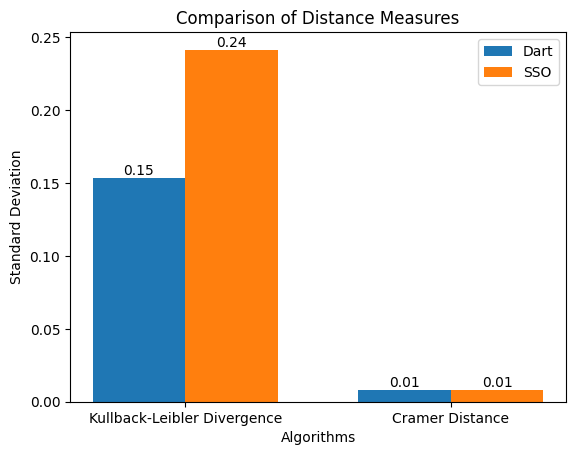
\includegraphics[width=0.8\textwidth]{5 Results/Figures/5.2 Bar Chart.png}
    \caption{Pop-Share Distance Measure}
    \label{fig:pop-share-distance-measure}
\end{figure}

As shown in Figure \ref{fig:pop-share-distance-measure}, our Dart implementation of Kullback-Leibler Divergence (KLD) demonstrates a standard deviation of 0.15, which is lower than the Python implementation’s standard deviation of 0.24. Both implementations incorporate a small epsilon value of $1.0e-12$ to address cases where either p or q are zero. The minimal variance of 0.09 in the Dart implementation suggests that our implementation exhibits less fluctuation compared to the Python implementation, indicating greater stability and consistency in its distance measure calculations.

For Cramer's Distance (CD), the standard deviation was the same for both implementations at 0.1. This finding aligns with our hypothesis that we should observe the same or very small amounts of variance between the two implementations, further supporting the reliability of the Dart implementation in maintaining consistency across distance measure calculations.
